\chapter[Event Displays][Event Displays]{Event Displays}
\label{app:eventdisplays}
\begin{figure}[h]
    \centering
    \makebox[\textwidth][c]{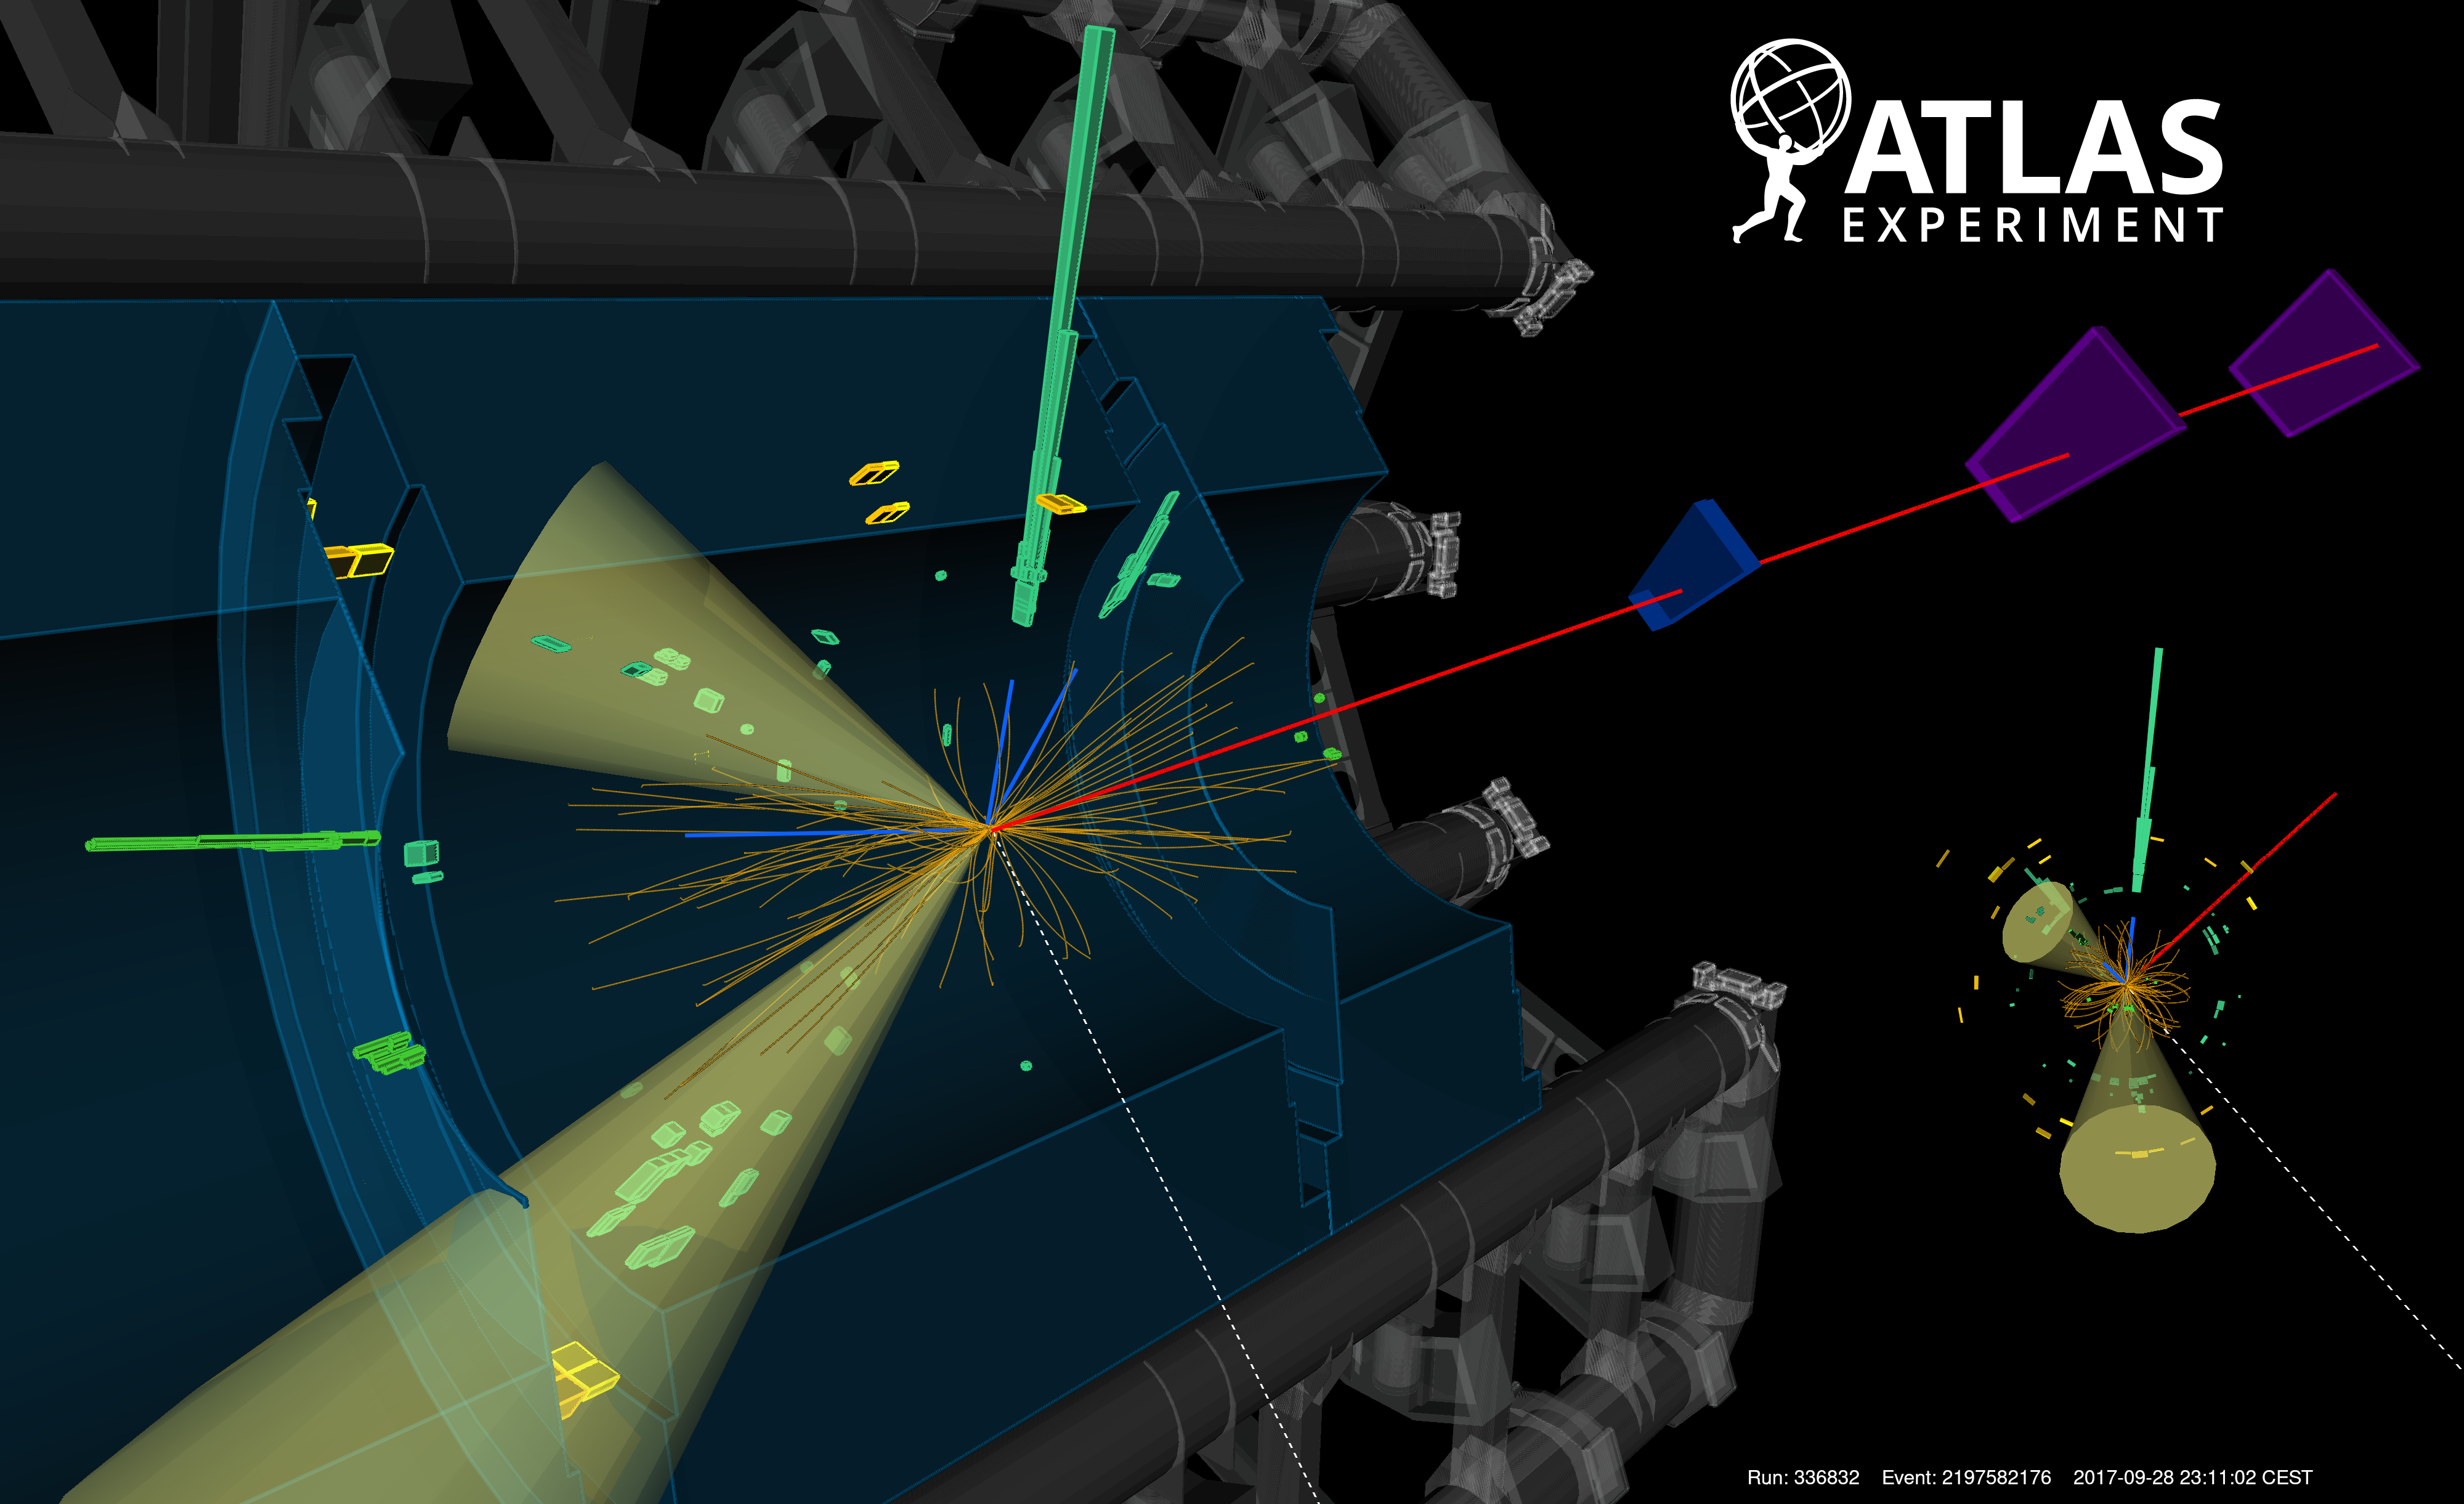
\includegraphics[width=1.2\textwidth]{figs/rpvthreel/SRFR.png}}
    %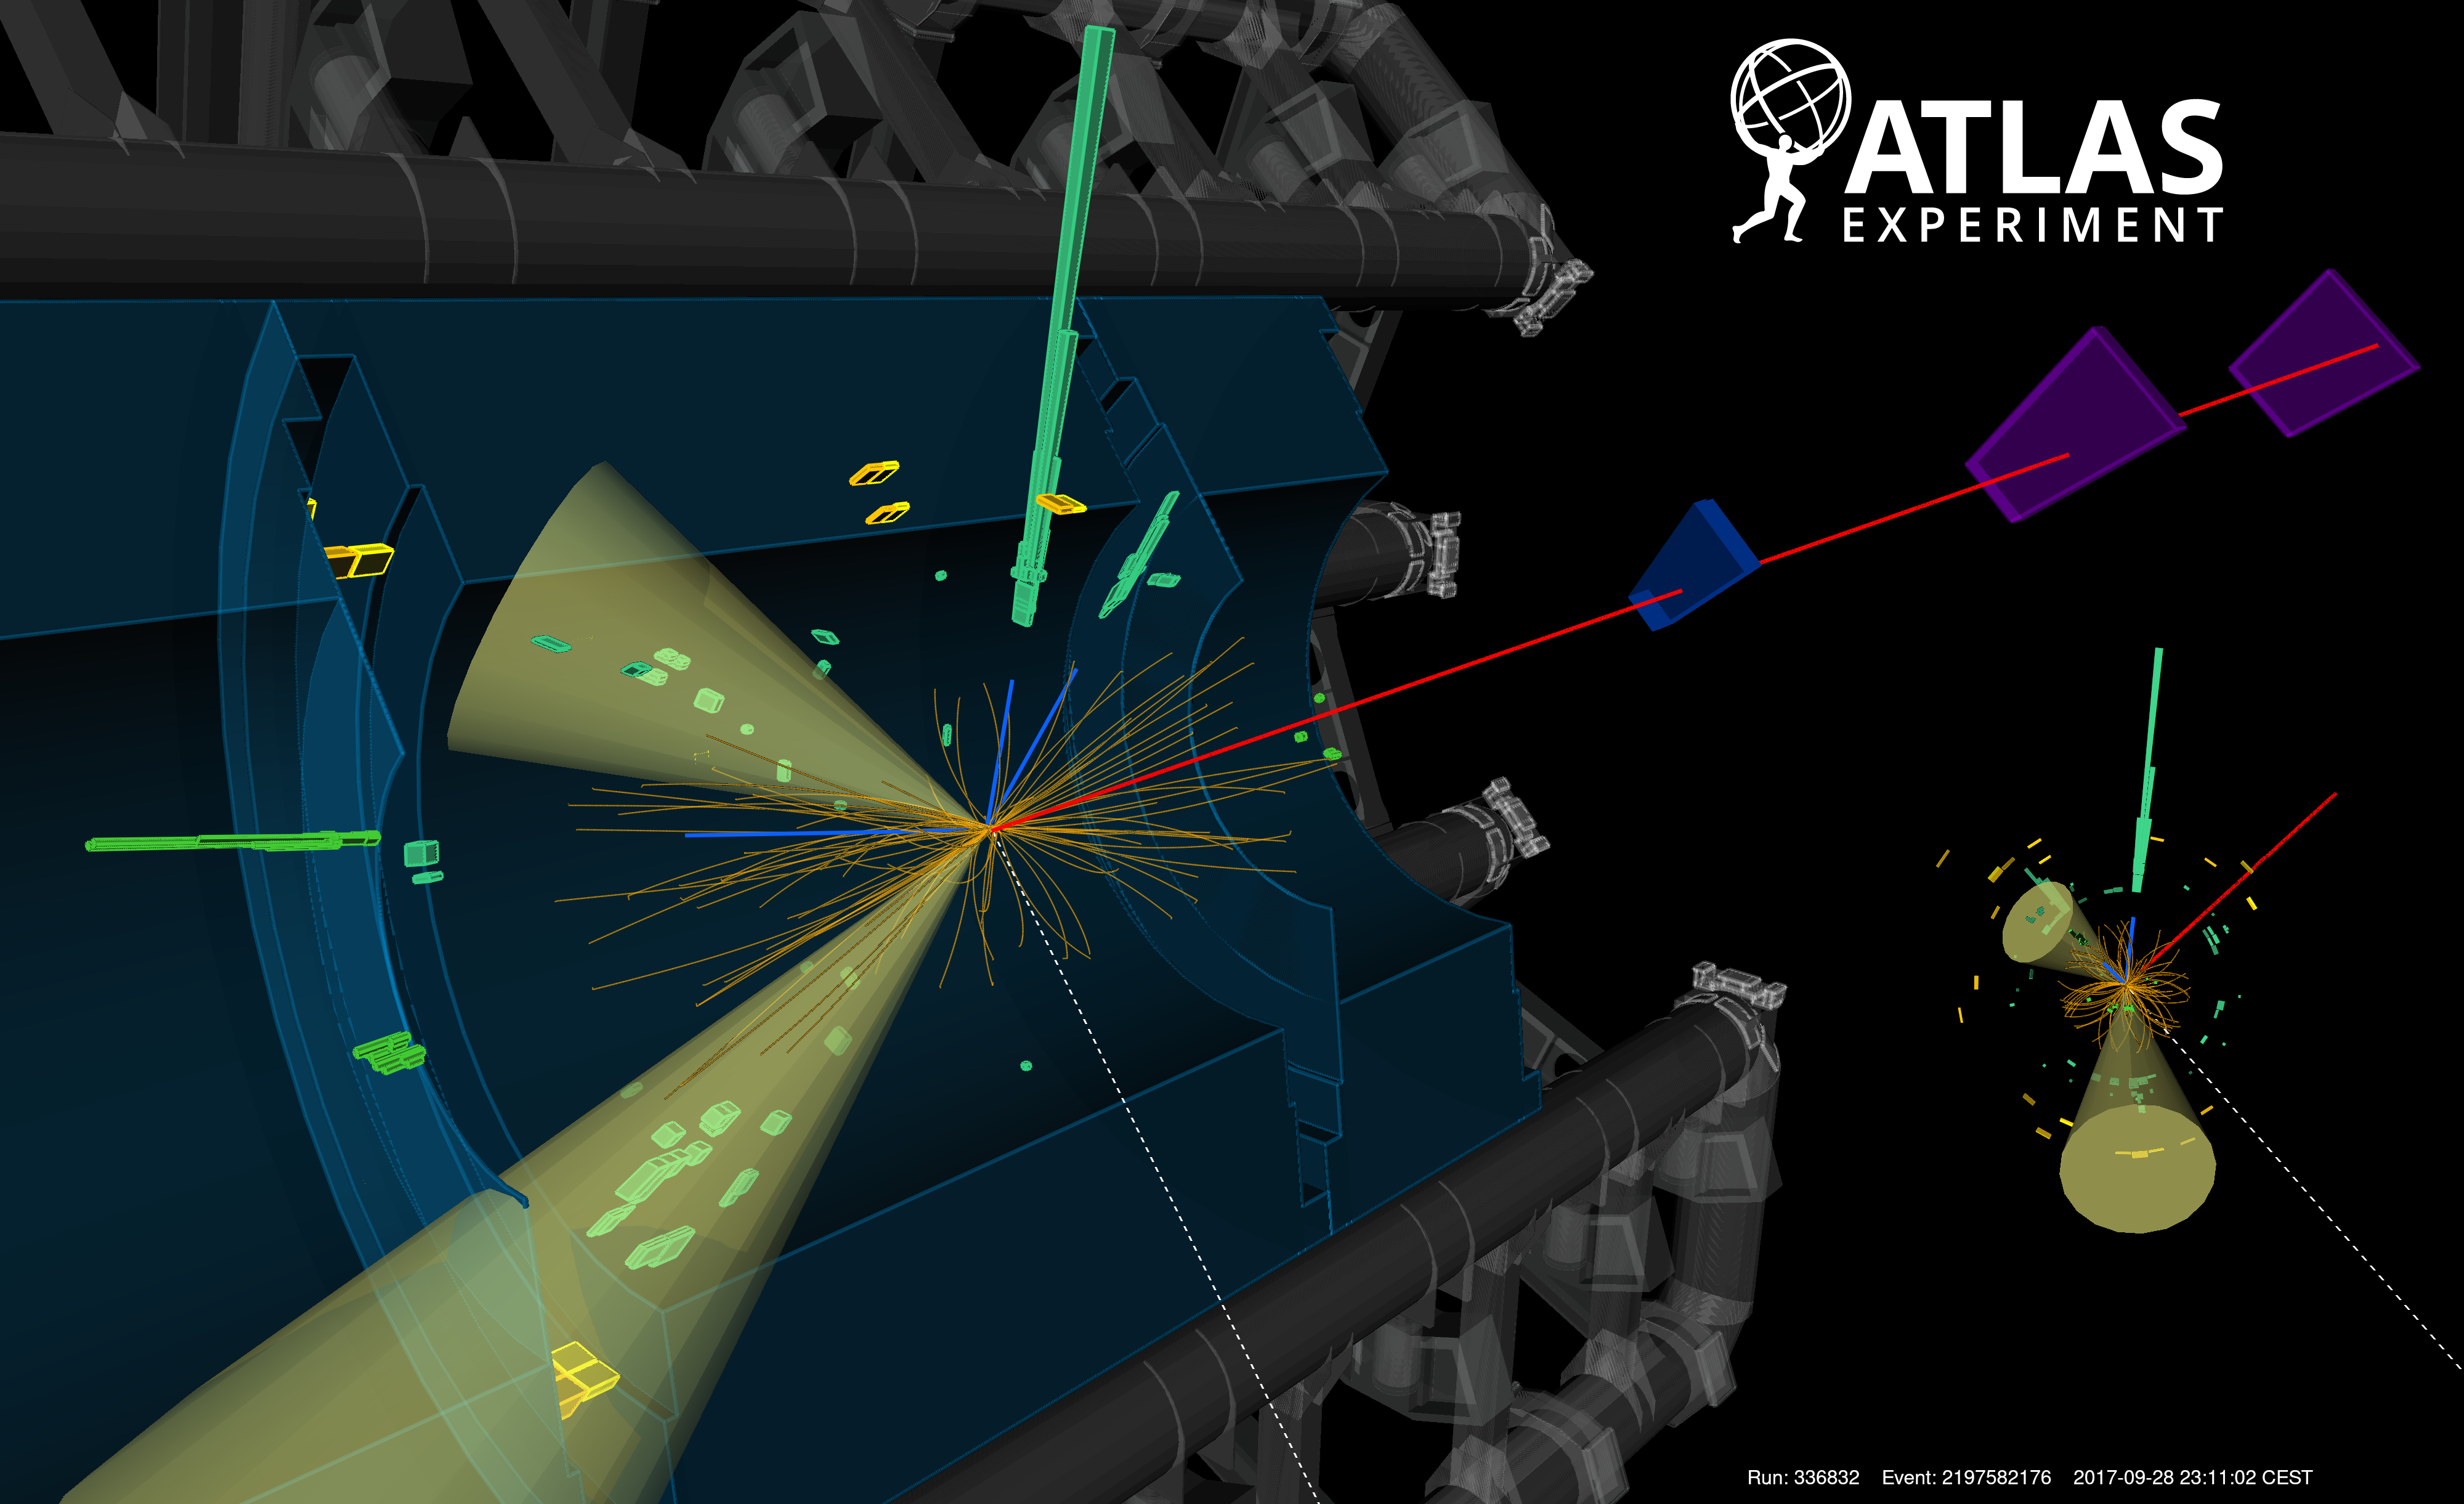
\includegraphics[width=1.00\textwidth]{figs/rpvthreel/SRFR.png}
    \caption[Event display for data event in the \SRFR signal region]{ The event display shows a data event recorded in September of 2017 which falls into the fully reconstructed signal region (\SRTL).
    The event consists of three electrons (blue lines), one muon (red line)  and two jets (yellow cones), neither of which are $b$-tagged.
    Two electrons with kinematic properties (\pt, $\eta$, $\phi$) of (46.5~\GeV, 1.14, 0.52) and (61.8~\GeV, -2.14, 0.42) form an invariant mass of \mll= 93.2~\GeV, consistent with a $Z$ boson.
    They are paired with a third electron (103.4~\GeV, 0.09, 1.31), with \mZl= 365.8~\GeV.
    The first jet (77.9~\GeV, -1.17, -2.00) and second jet (32.3~\GeV, -0.76, 0.26) are used to reconstruct a second $Z$ boson candidate of \mjj= 94.7~\GeV.
    The jets are paired with the muon (44.7~\GeV, 2.33, 2.04), with \mZl = 403.0~\GeV.
    The event has a missing transverse energy of \met = 116.49~\GeV, which is represented as a dashed white line at $\phi=-2.40$~\cite{ATLAS:2020uer}.}
    \label{fig:eventdisplaySRFR}
\end{figure}

\begin{figure}[h]
    \centering
    \makebox[\textwidth][c]{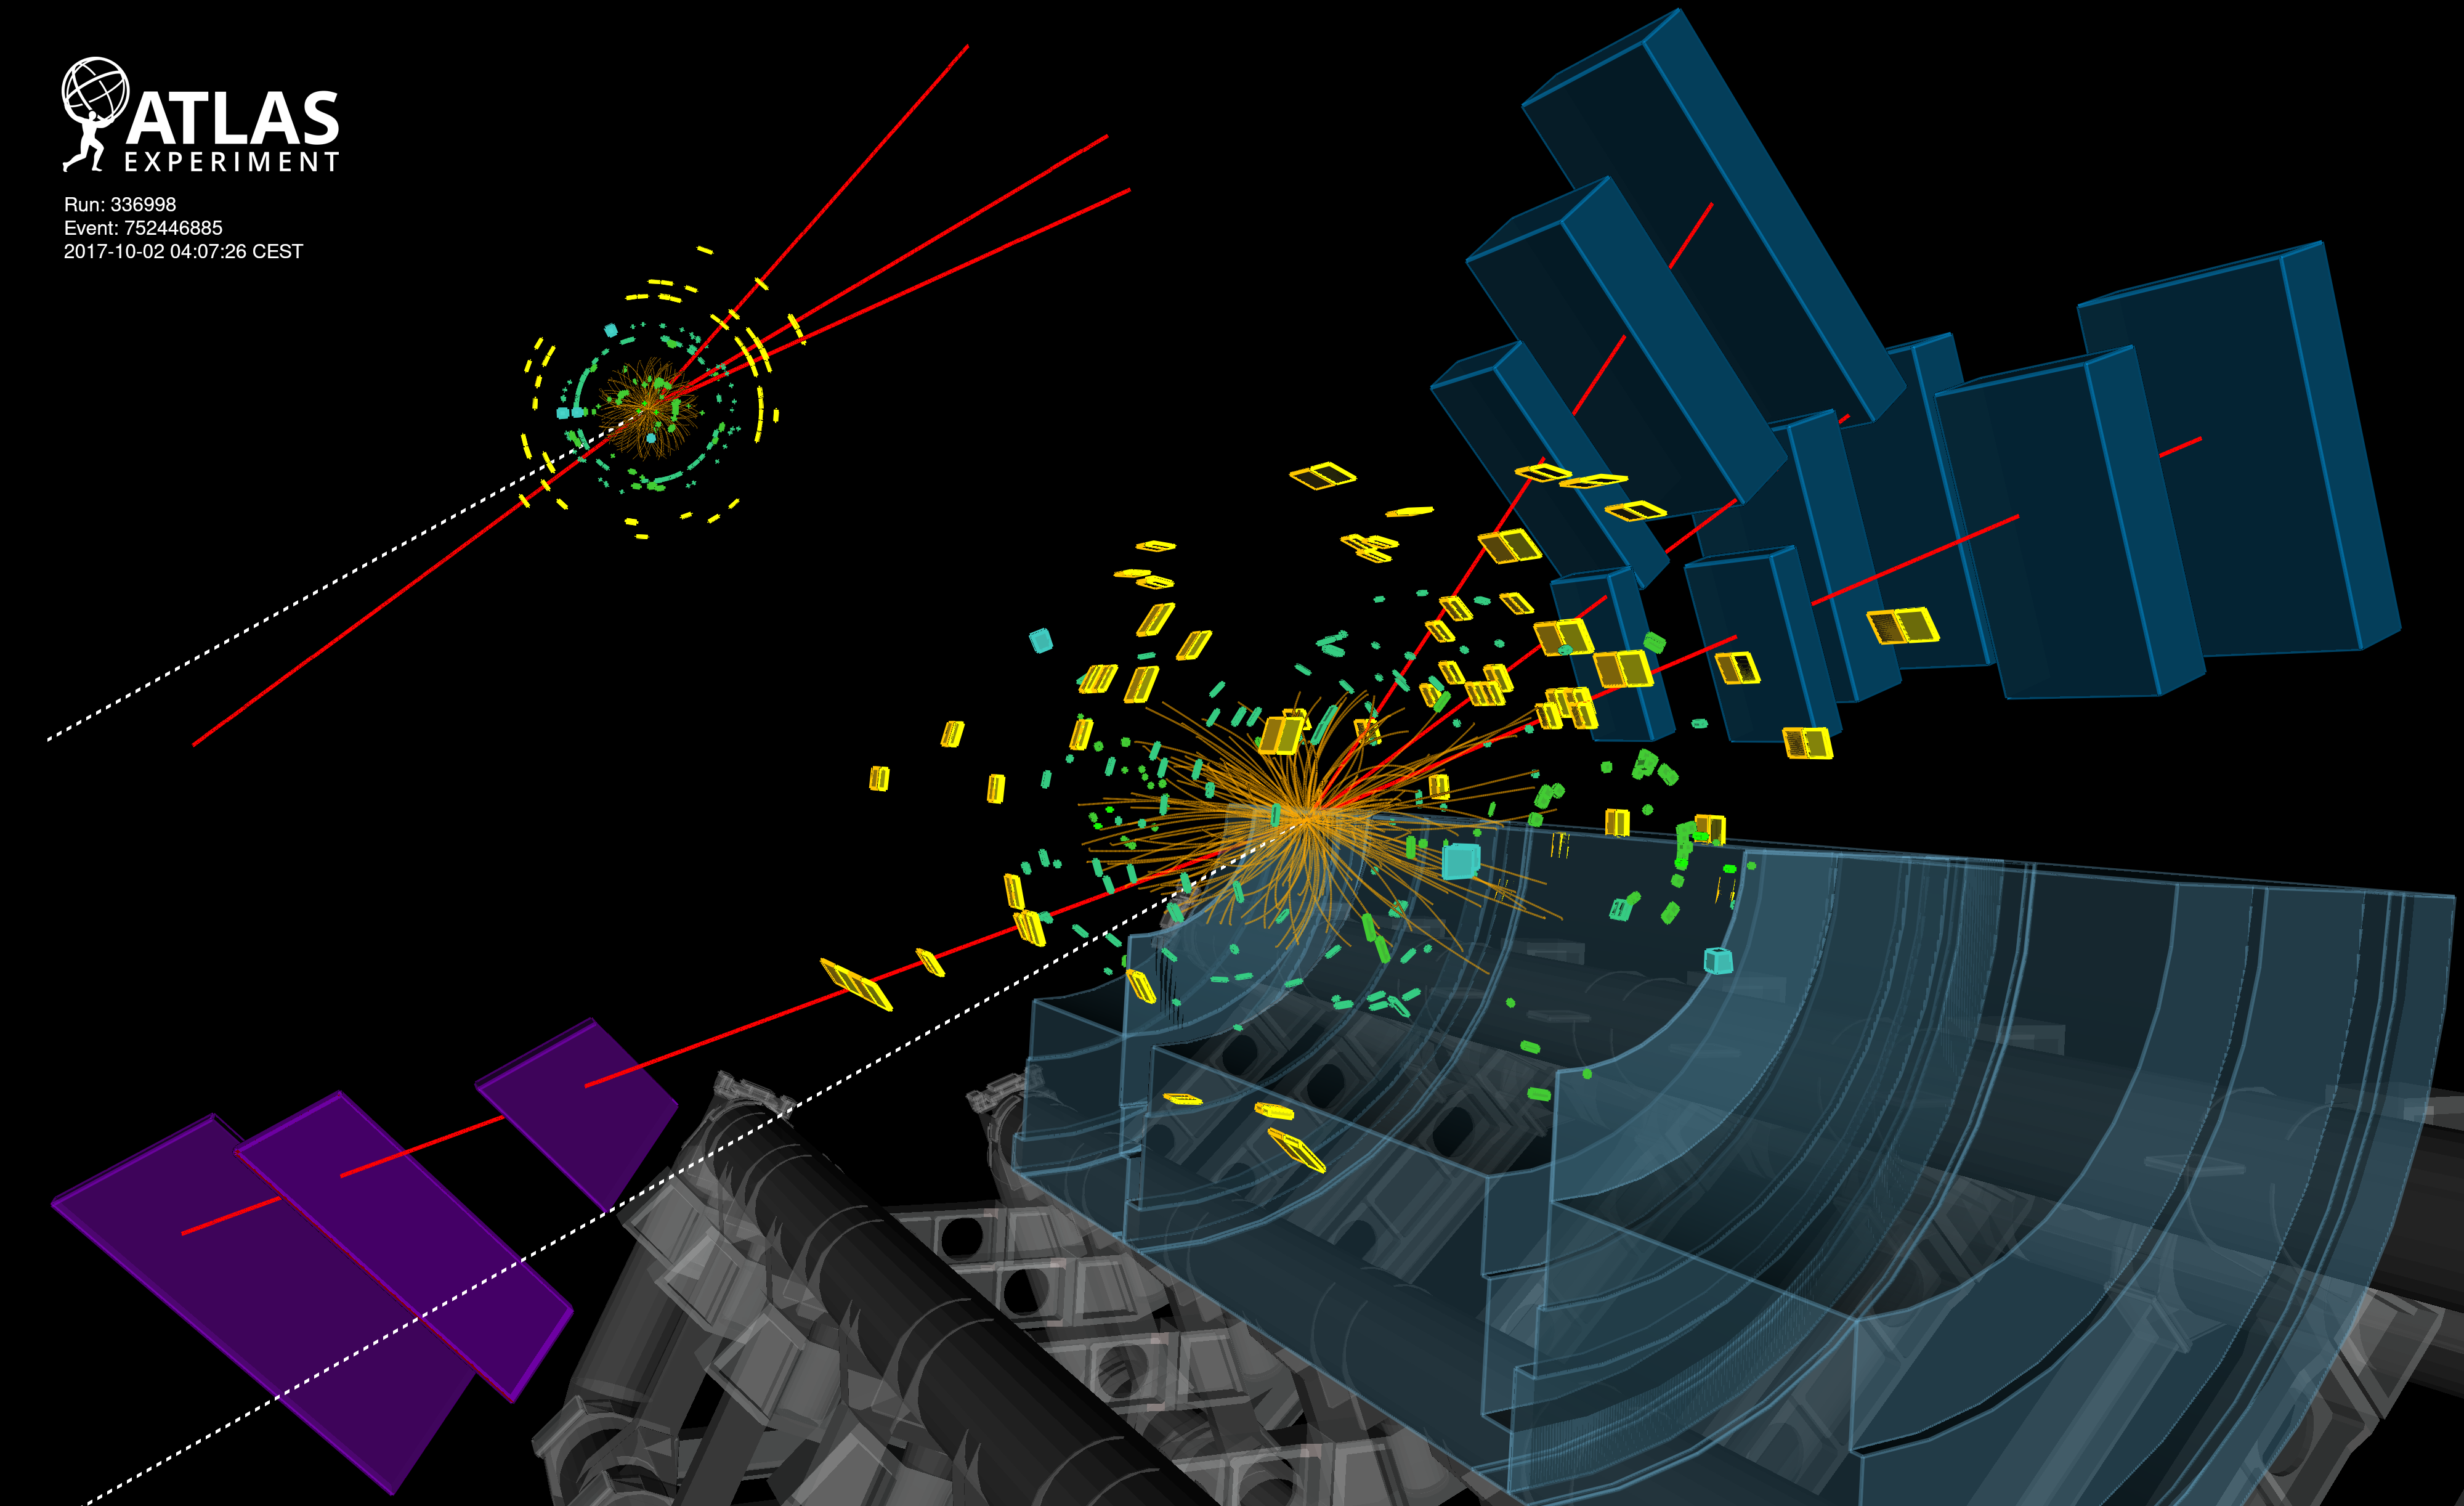
\includegraphics[width=1.2\textwidth]{figs/rpvthreel/SR4l.png}}
    %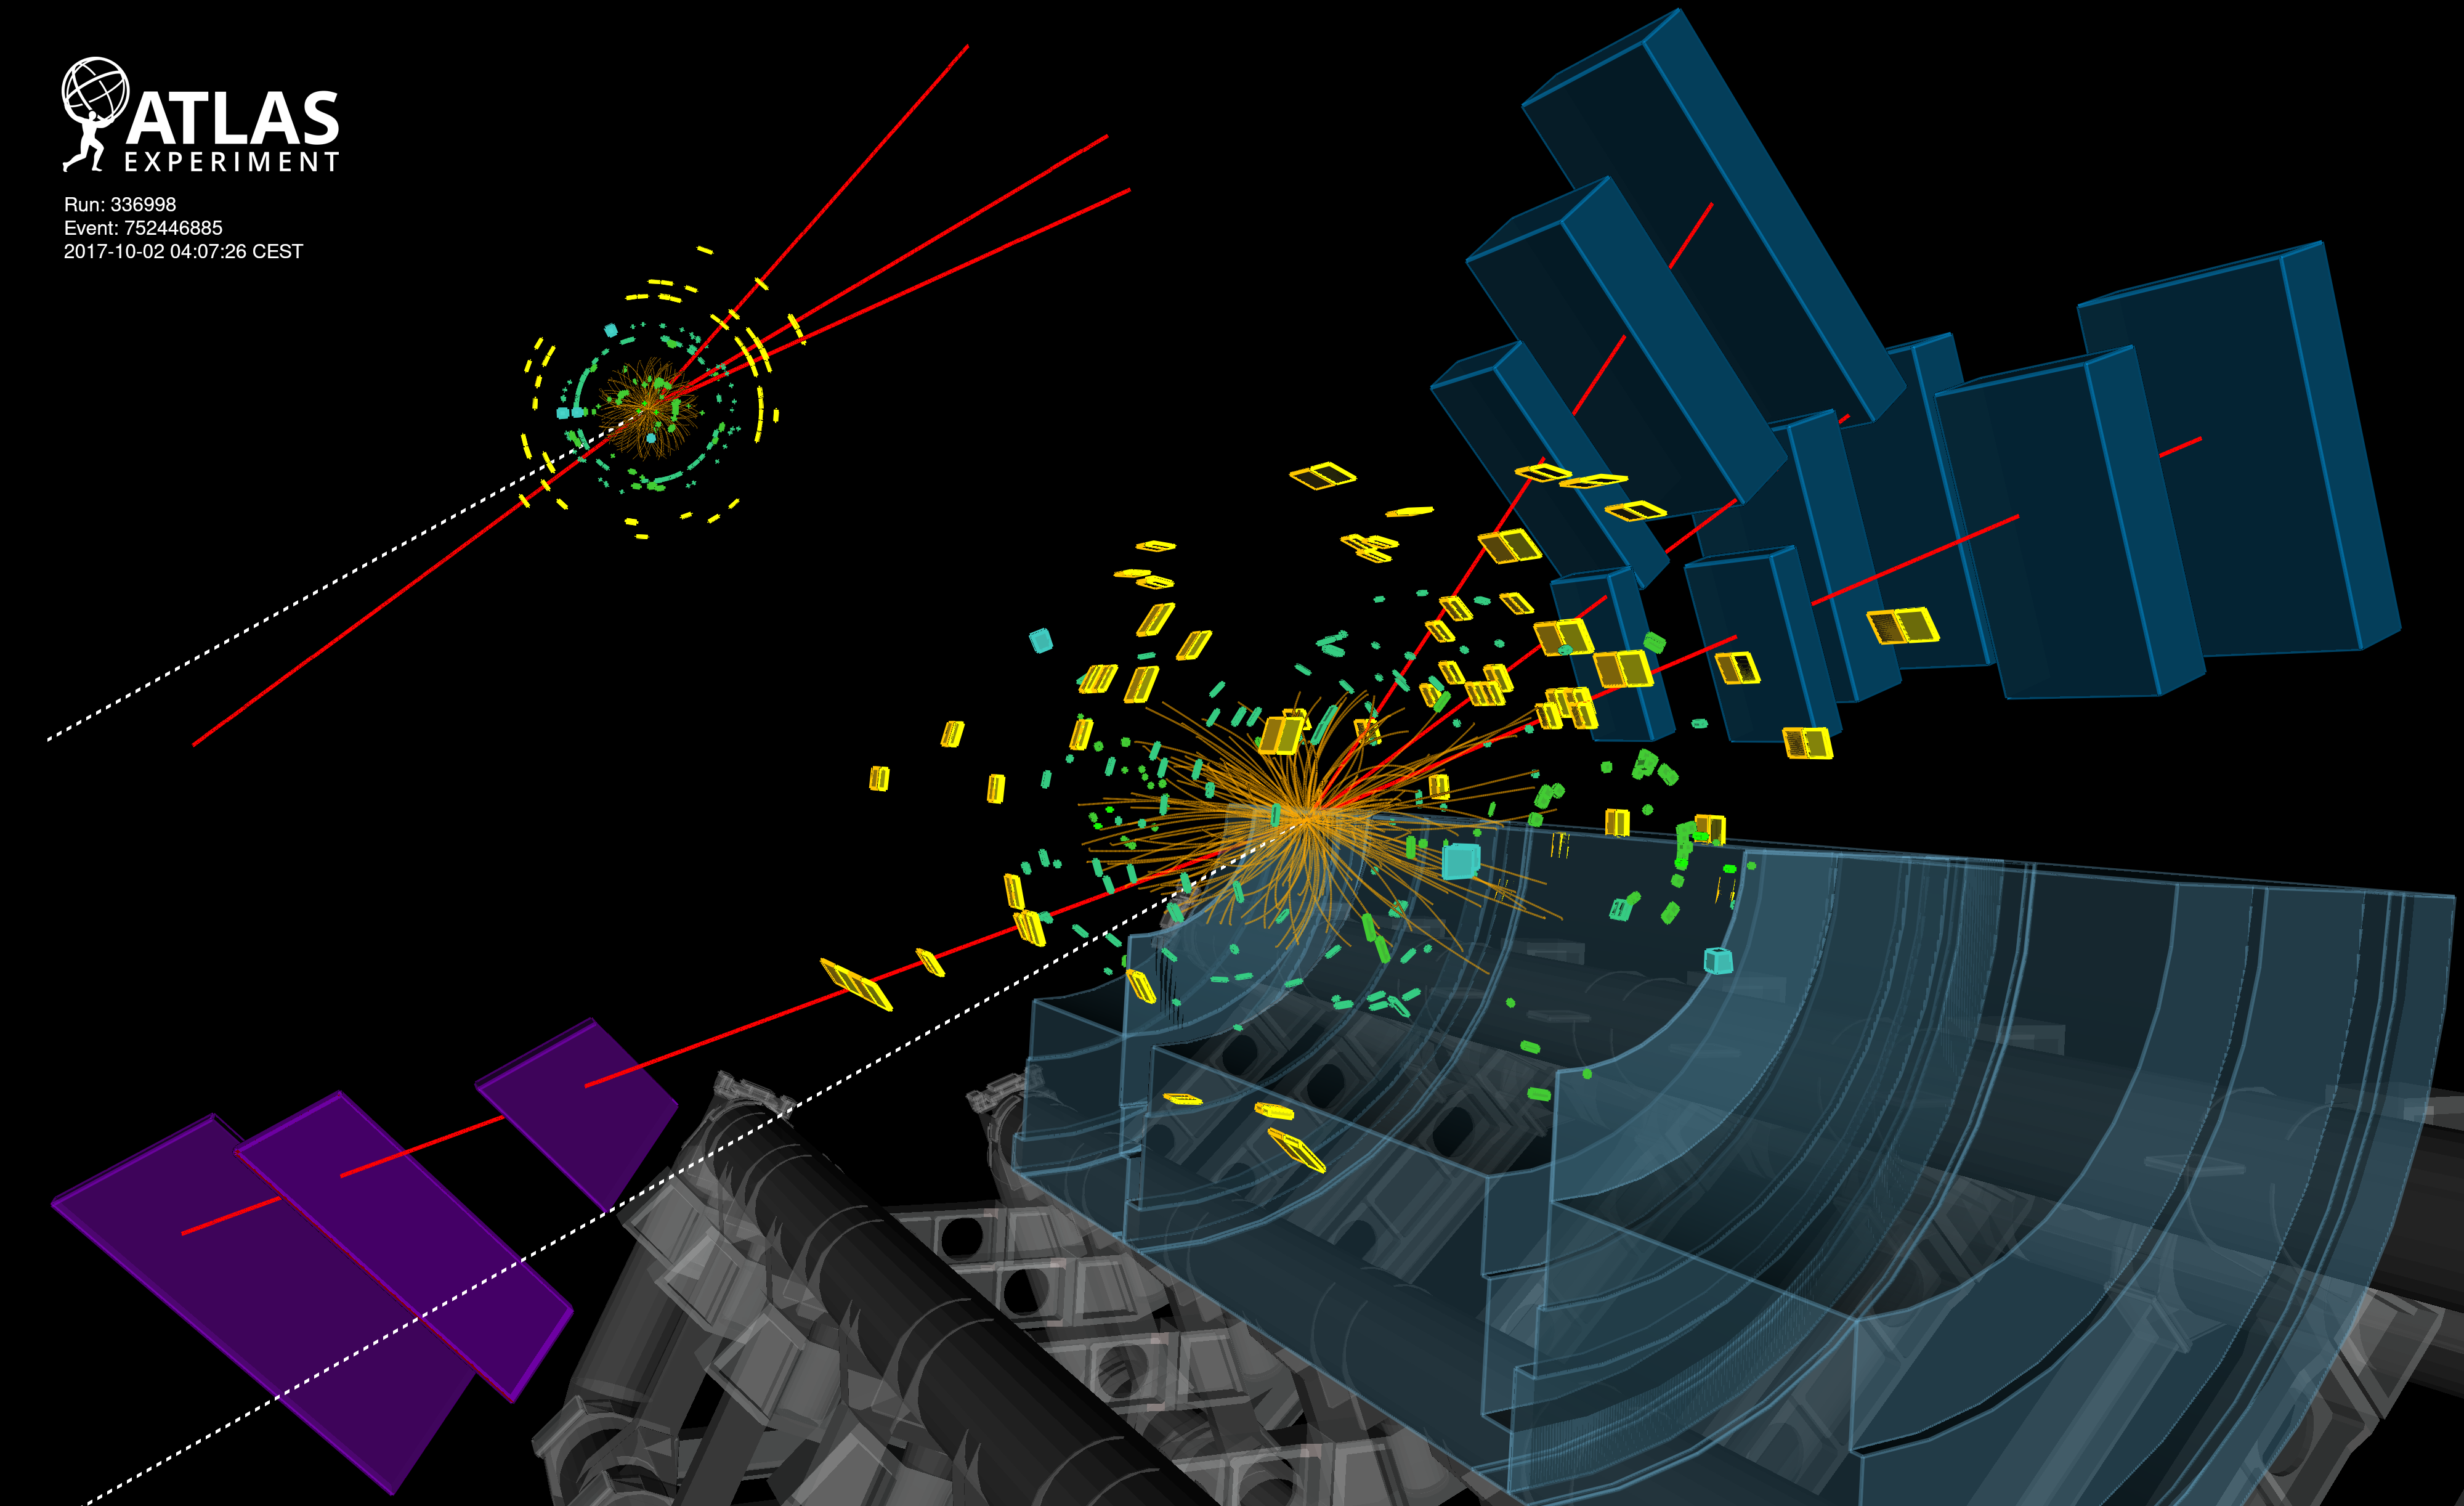
\includegraphics[width=1.00\textwidth]{figs/rpvthreel/SR4l.png}
    \caption[Event display for data event in the \SRFour signal region]{The event display shows a data event recorded in October of 2017 which falls into the four lepton signal region (\SRFour).
    This event consists of four muons (red lines). 
    Two muons with kinematic properties (\pt, $\eta$, $\phi$) of (179.0~\GeV, -0.26, 0.53) and (292.9~\GeV, 0.10, 0.43) form an invariant mass of \mll= 88.4~\GeV, consistent with a $Z$ boson.
    They are paired with a third muon (206.8~\GeV, -1.08, -2.50), with \mZl= 719.4~\GeV.
    There is a fourth muon (126.6~\GeV, -0.29, 0.85) that is unpaired.
    The event has a missing transverse energy of \met= 390.6~\GeV, which is represented as a dashed white line at $\phi=-2.66$. \cite{ATLAS:2020uer}}
    \label{fig:eventdisplaySR4l}
\end{figure}
\begin{figure}[ht]
    \centering
    \makebox[\textwidth][c]{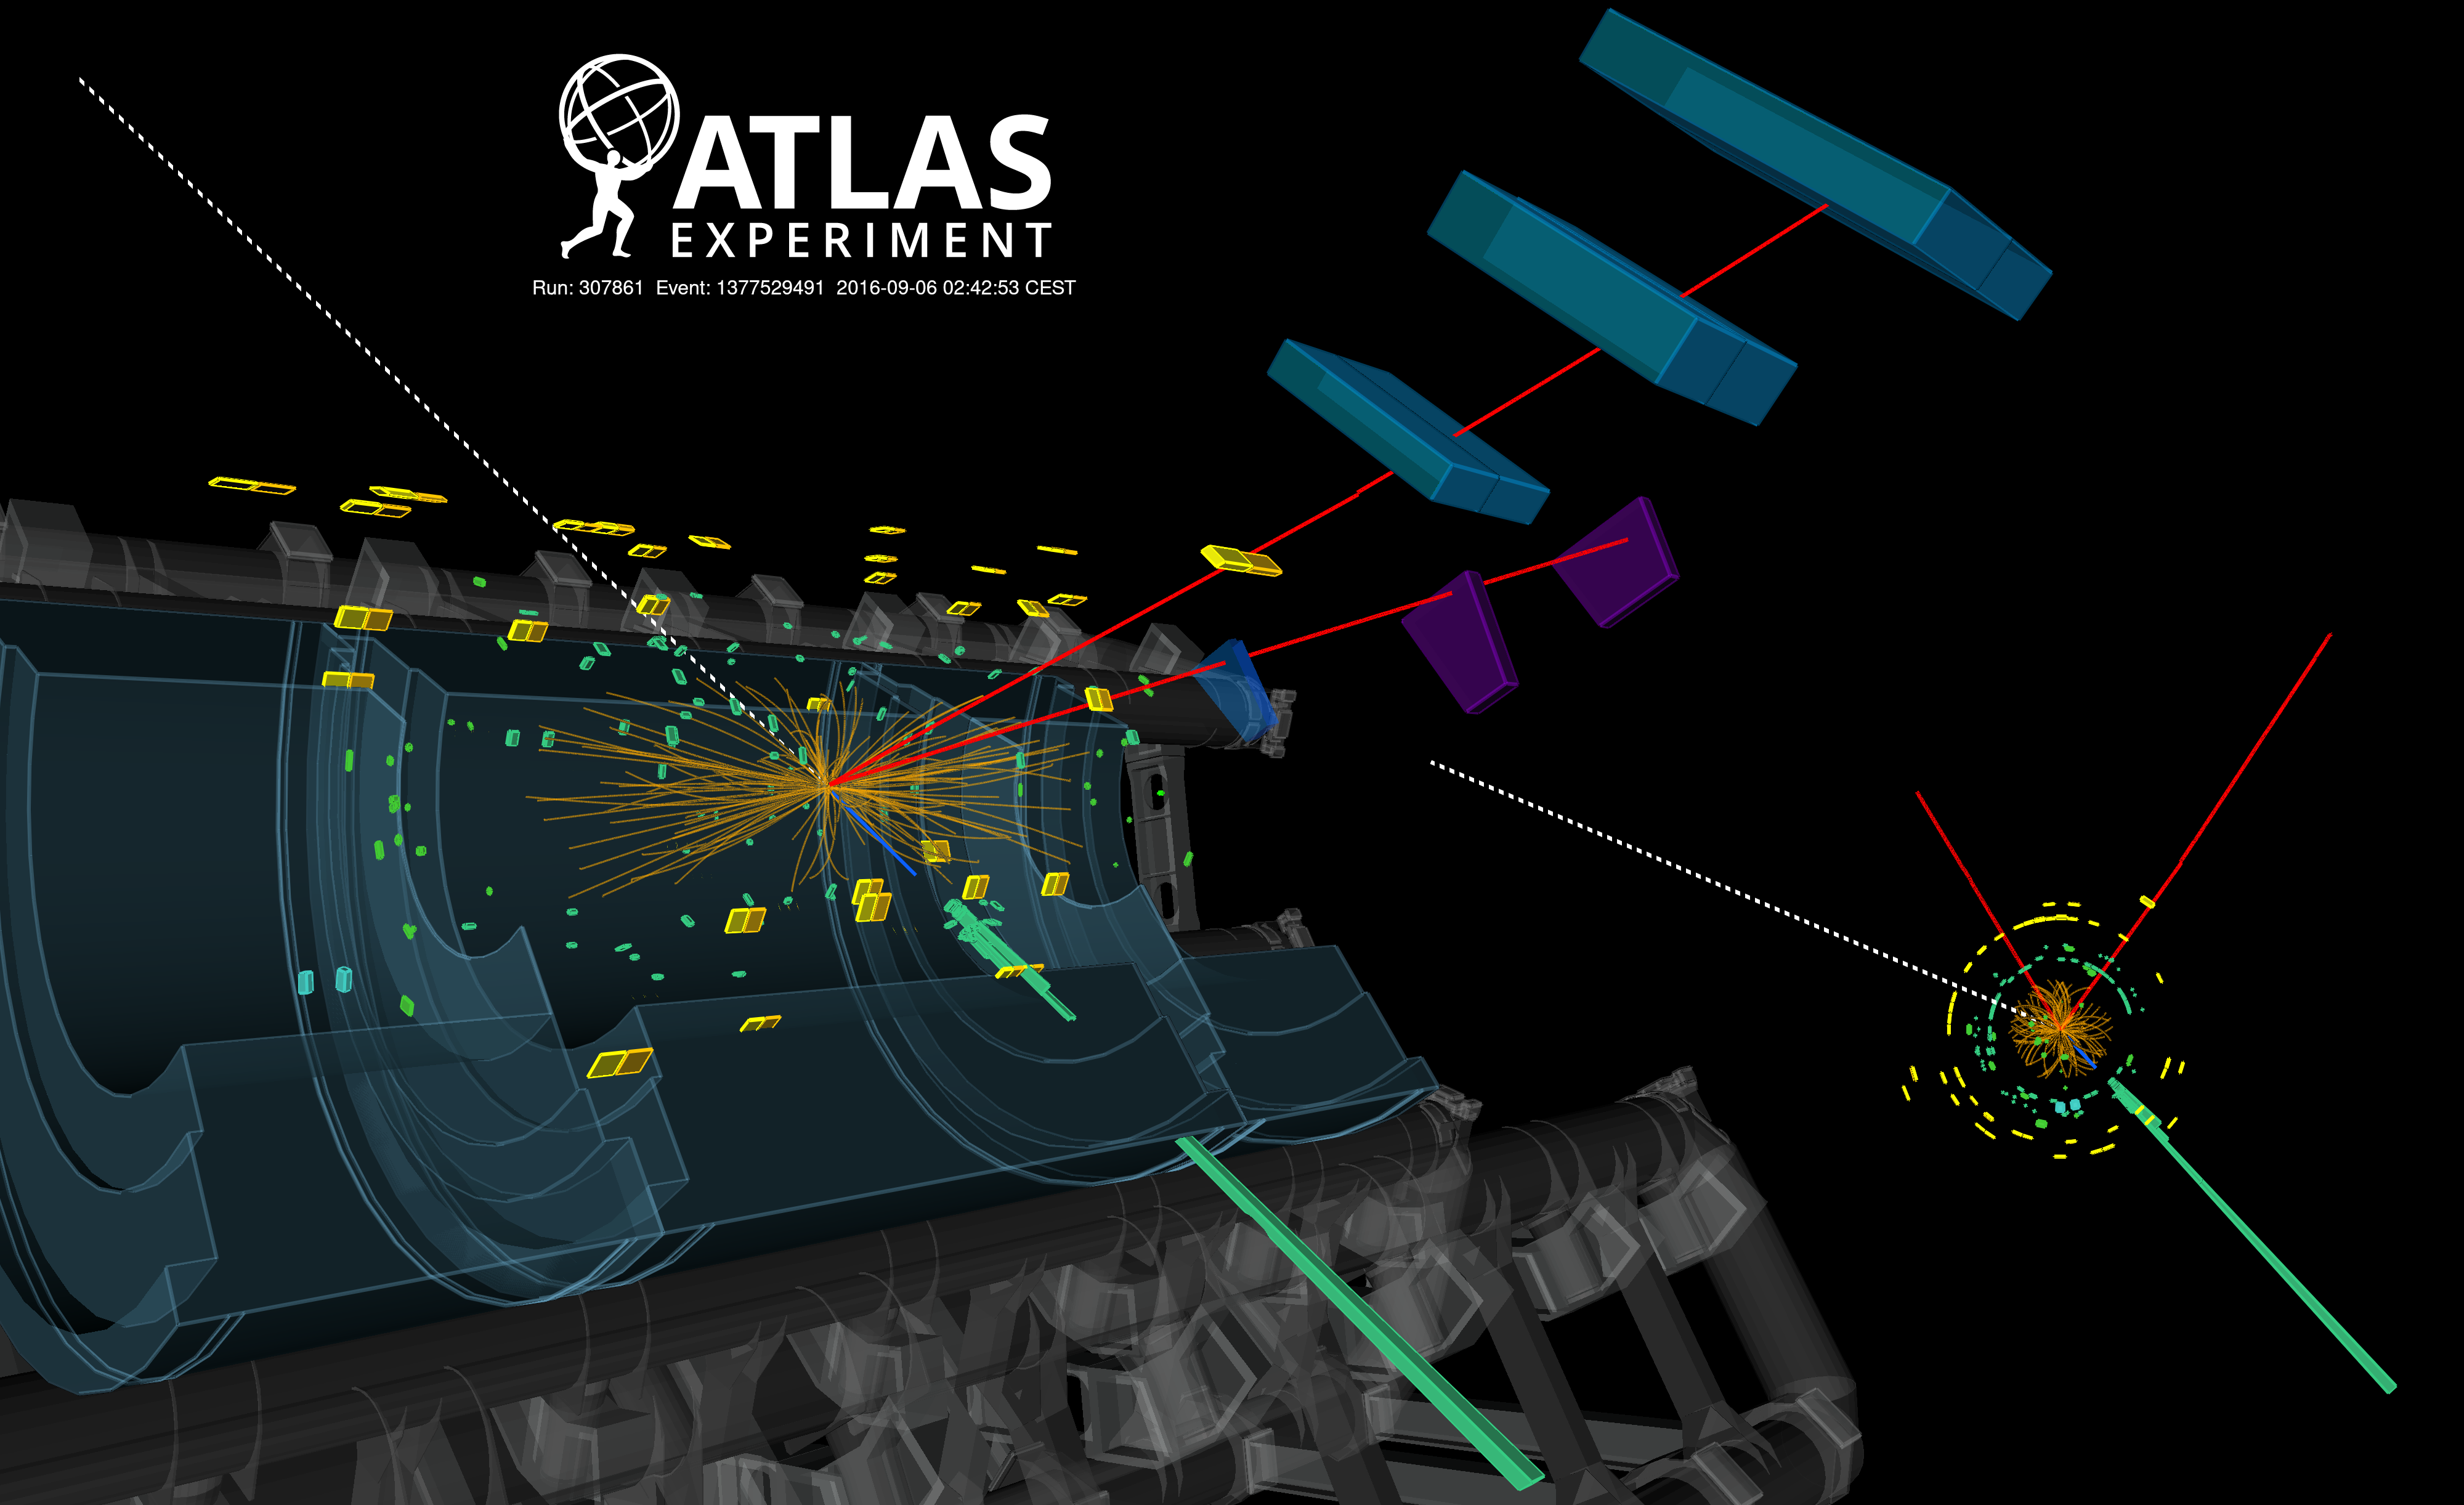
\includegraphics[width=1.2\textwidth]{figs/rpvthreel/SR3l.png}}
    %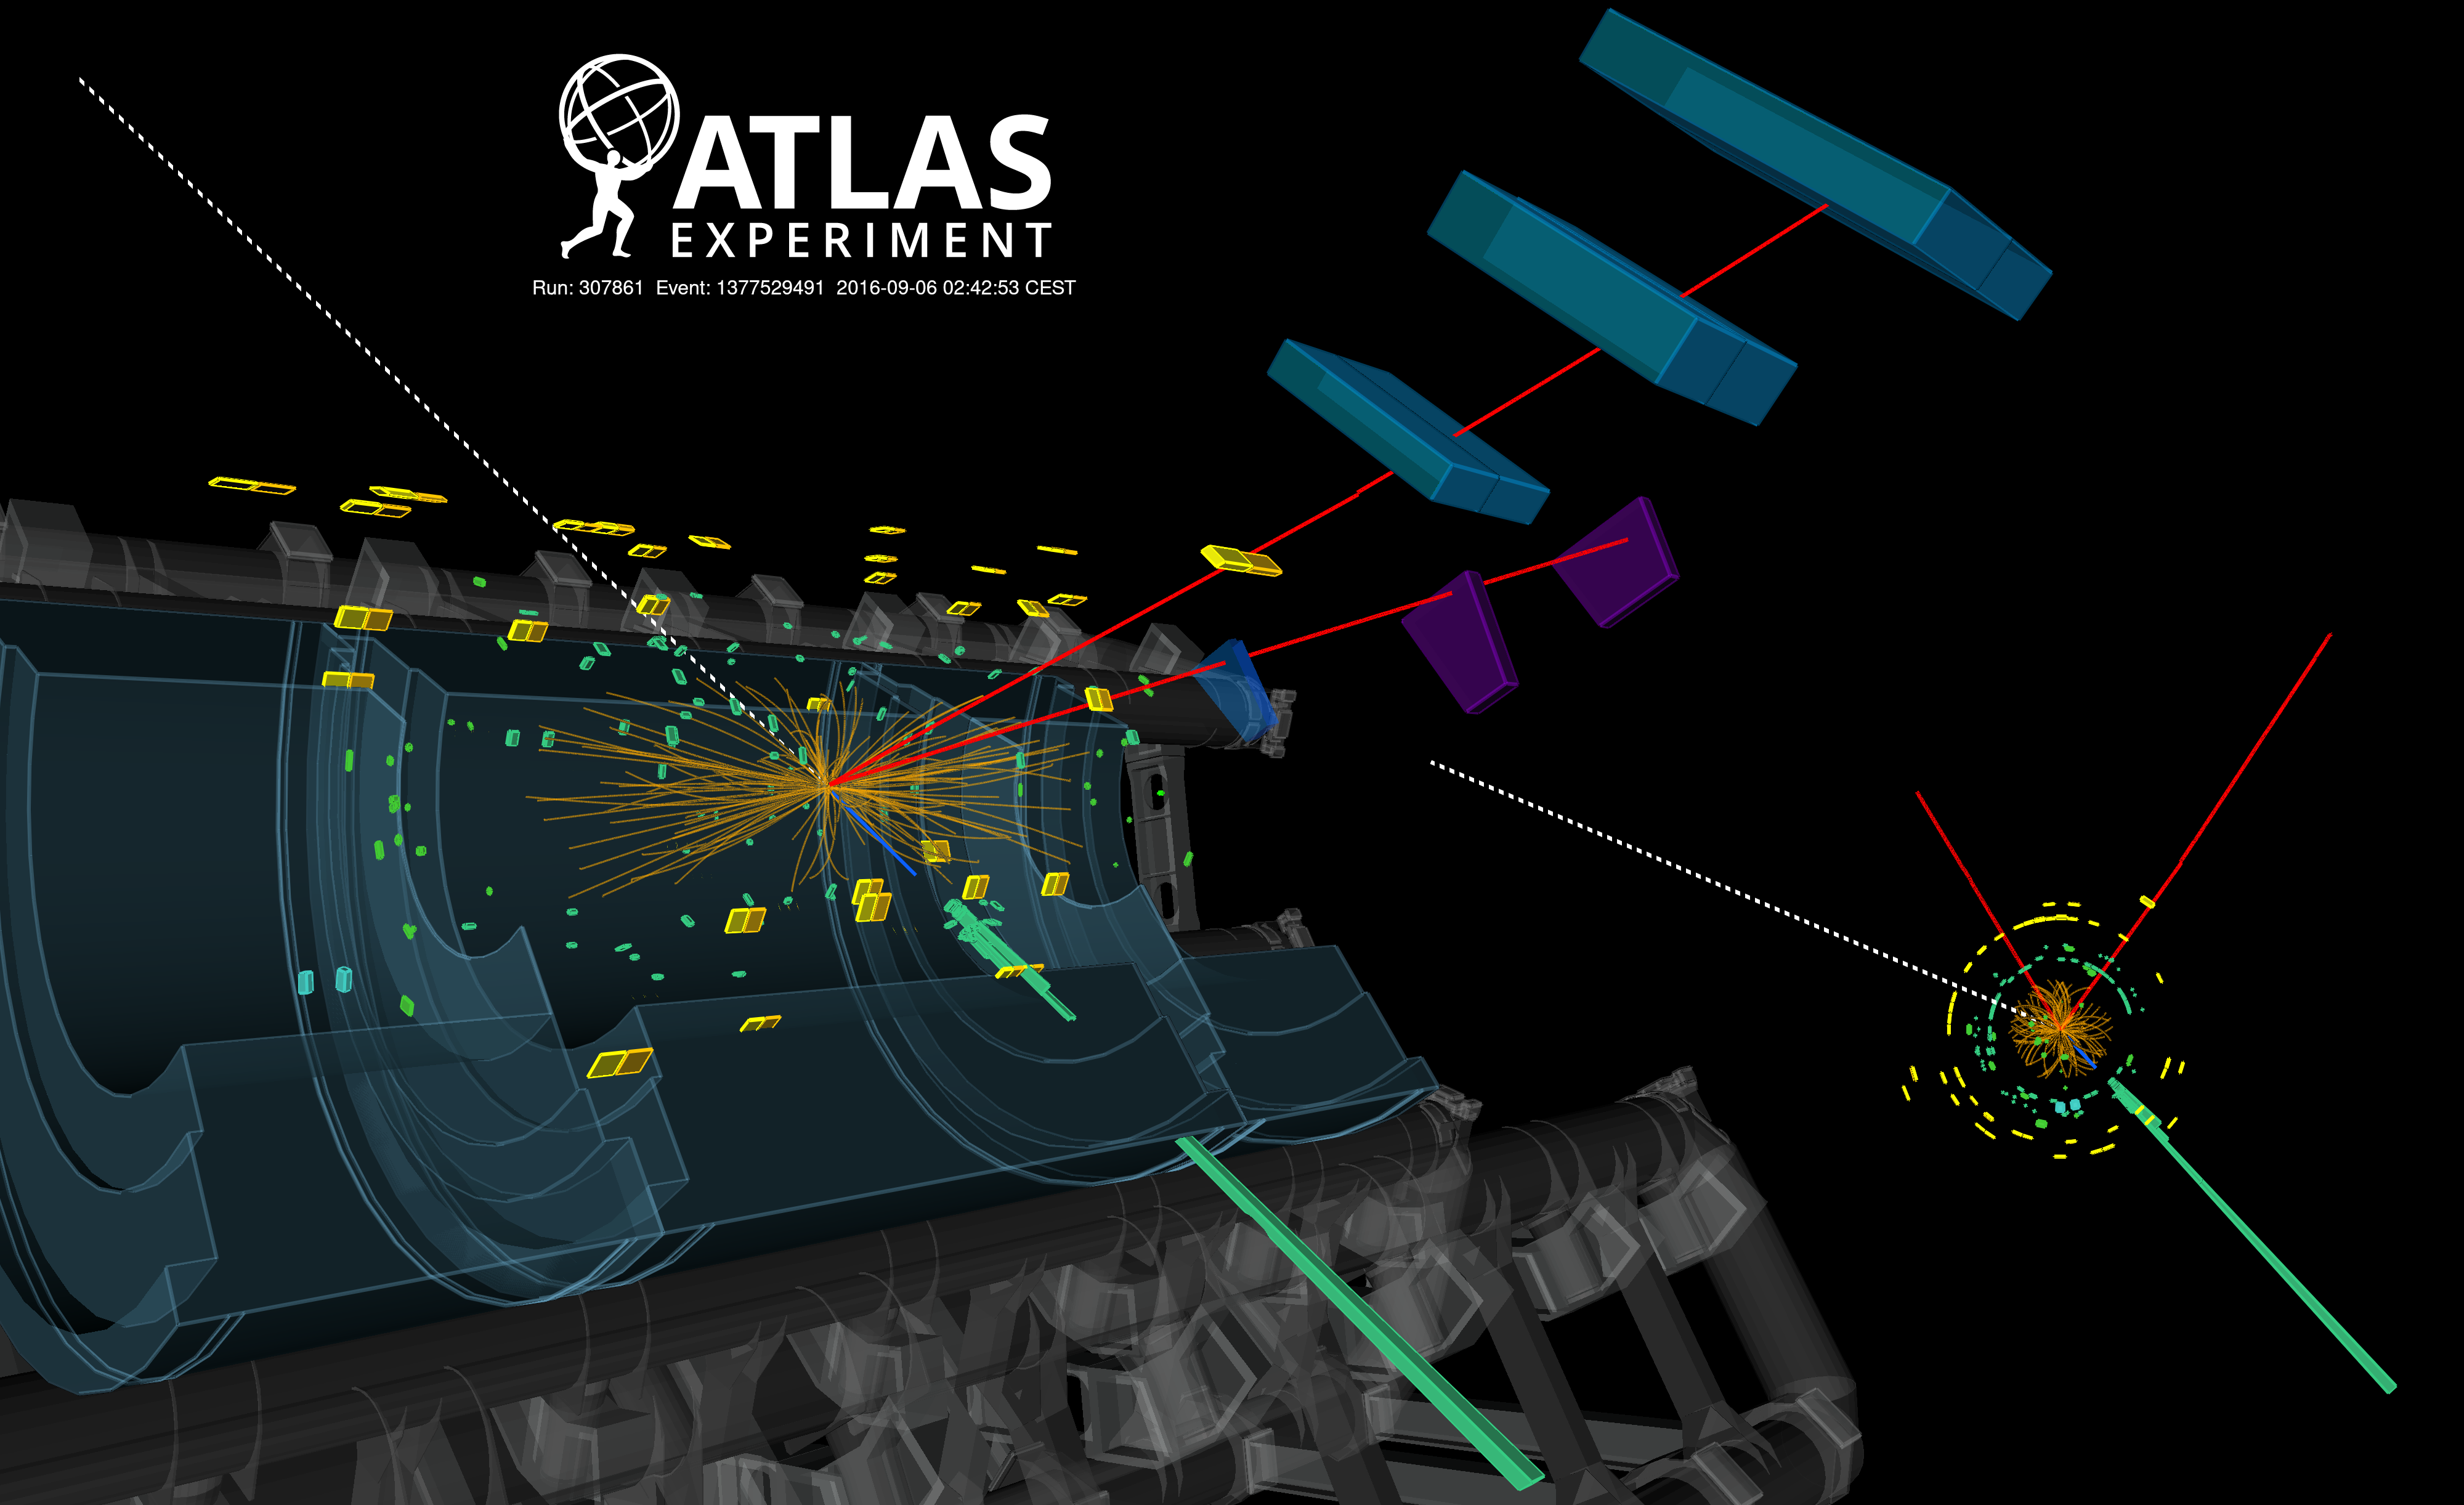
\includegraphics[width=1.00\textwidth]{figs/rpvthreel/SR3l.png}
    \caption[Event display for data event in the \SRThree signal region]{The event display shows a data event recorded in September of 2016 which falls into the three lepton signal region (\SRThree). This event consists of two muons (red lines) and one electron (blue line).
    The muons with kinematic properties (\pt, $\eta$, $\phi$) of (217.0~\GeV, -2.05, 1.87) and (14.4~\GeV, -0.97, 0.74) form an invariant mass of of \mll= 87.0~\GeV, consistent with a $Z$ boson.
    The muons are paired with the electron (362.2~\GeV, -0.53, -1.06), with \mZl=  742.7~\GeV.
    The event has a missing transverse energy of \met= 172.5~\GeV, which is represented as a dashed white line at $\phi=2.51$. \cite{ATLAS:2020uer}}
    \label{fig:eventdisplaySR3l}
\end{figure}